% exercise sheet with header on every page for math or close subjects
\documentclass[12pt]{article}
\usepackage[utf8]{inputenc}
\usepackage{latexsym}
\usepackage{multicol}
\usepackage{fancyhdr}
\usepackage{amsfonts}
\usepackage{amsmath}
\usepackage{amssymb}
\usepackage{enumerate}
\usepackage{listings}
\usepackage{graphicx}

% Shortcuts for bb, frak and cal letters
\newcommand{\E}{\mathbb{E}}
\newcommand{\V}{\mathbb{V}}
\renewcommand{\P}{\mathbb{P}}
\newcommand{\N}{\mathbb{N}}
\newcommand{\R}{\mathbb{R}}
\newcommand{\C}{\mathbb{C}}
\newcommand{\Z}{\mathbb{Z}}
\newcommand{\Pfrak}{\mathfrak{P}}
\newcommand{\Pfrac}{\mathfrak{P}}
\newcommand{\Bfrac}{\mathfrak{P}}
\newcommand{\Bfrak}{\mathfrak{B}}
\newcommand{\Fcal}{\mathcal{F}}
\newcommand{\Ycal}{\mathcal{Y}}
\newcommand{\Bcal}{\mathcal{B}}
\newcommand{\Acal}{\mathcal{A}}

% formating
\topmargin -3.5cm
\textheight 22cm
\textwidth 16.0 cm
\oddsidemargin -0.1cm

% Fancy Header on every Page
\pagestyle{fancy}
\lhead{\textbf{Embedded Systems Milestone 2}}
\rhead{Daniel Schäfer (2549458)\\ Rafael Dewes (2548365)\\ Kevin M\"uller (2550062)}
\renewcommand{\headrulewidth}{1.2pt}
\setlength{\headheight}{110pt}

\begin{document}
\pagenumbering{gobble}
\lstset{language=C++}

\section*{Important Notes}

\subsection*{The GUI and how to install/use it}
\url{https://github.com/kvnmlr/simulink-advanced-visualization/releases}
to download our GUI (Created using Unity)\\

We decided to use a GUI built in unity, because it made it significantly easier to observe the game and the sending of data using TCP Blocks did not impact performance significantly.

The GUI has to be started before starting the simulation (using \verb!model.slx!)

\section*{Our Submission Scenarios}
put Seeds etc here and explain what happens

\section*{Collision}
TODO explain what works, whats missing

\section*{Push conditions to avoid scout}
The condition is implemented (and working), but because our Collision is not completely implemented yet, the impossible case of the hitboxes of collector and scout overlapping will cause our collector to not detect the scout of our team correctly.\\

The detection works as shown below:\\
\begin{center}
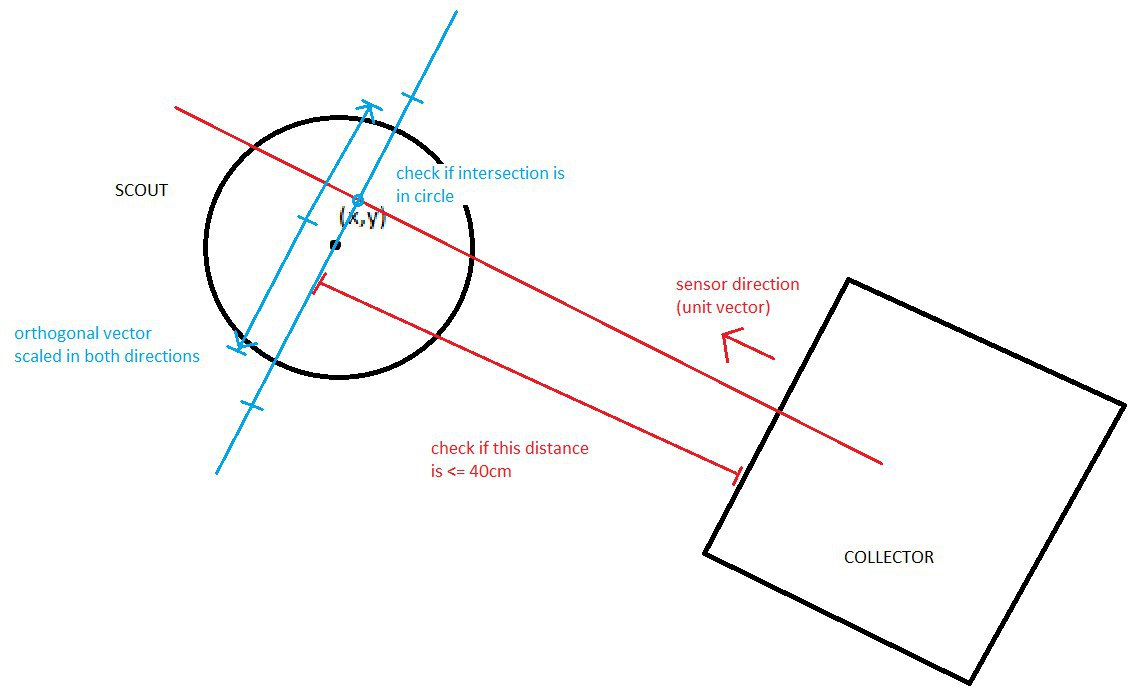
\includegraphics[scale = 0.4]{pictures/scout_condition}
\end{center}


\end{document}
